\documentclass[a4paper, 12pt]{article}

\usepackage[portuges]{babel}
\usepackage[utf8]{inputenc}
\usepackage{amsmath}
\usepackage{indentfirst}
\usepackage{graphicx}
\usepackage{multicol,lipsum}
\usepackage{booktabs}
\usepackage{longtable}
\usepackage{graphicx}
\usepackage{pst-pdf}
\usepackage{listings}
\usepackage{xcolor}
\lstset { %
	language=C++,
	backgroundcolor=\color{black!5}, % set backgroundcolor
	basicstyle=\footnotesize,% basic font setting
}

\begin{document}
	%\maketitle
	
	\begin{titlepage}
		\begin{center}
			
			%\begin{figure}[!ht]
			%\centering
			%\includegraphics[width=2cm]{c:/ufba.jpg}
			%\end{figure}
			
			\large{Társila Samille Santos da Silveira}\\ 
			\vspace{155pt}
			\vspace{95pt}
			\textbf{\LARGE{Relatório sobre Tabelas de Dispersão }}\\
			%\title{{\large{Título}}}
			\vspace{3,5cm}
		\end{center}
		
		
		
		
		\begin{center}
			\vspace{\fill}
			Brasil\\
			2020, v-1.0
		\end{center}
	\end{titlepage}
	%%%%%%%%%%%%%%%%%%%%%%%%%%%%%%%%%%%%%%%%%%%%%%%%%%%%%%%%%%%
	
	% % % % % % % % %FOLHA DE ROSTO % % % % % % % % % %
	
	\begin{titlepage}
		\begin{center}
			
			%\begin{figure}[!ht]
			%\centering
			%\includegraphics[width=2cm]{c:/ufba.jpg}
			%\end{figure}
			
			\large{Társila Samille Santos da Silveira}\\ 
			\vspace{15pt}
			
			\vspace{85pt}
			
			\textbf{\LARGE{Relatório sobre Tabelas de Dispersão}}
			\title{\large{Título}}
			%	\large{Modelo\\
			%   		Validação do modelo clássico}
			
		\end{center}
		\vspace{1,5cm}
		
		\begin{flushright}
			
			\begin{list}{}{
					\setlength{\leftmargin}{4.5cm}
					\setlength{\rightmargin}{0cm}
					\setlength{\labelwidth}{0pt}
					\setlength{\labelsep}{\leftmargin}}
				
				\item Relatório resumo apresentado à disciplina de Estrutura de Dados Básicas I, como requisito parcial para obtenção de nota referente à unidade III.
				
				
			\end{list}
		\end{flushright}
	\vspace{3cm}
\begin{center}{}
	
	
	
	\item Universidade Federal do Rio Grande do Norte - UFRN \
	\item Instituto Metrópole Digital - IMD \
	\item Bacharelado em Tecnologia da Informação\
	
\end{center}		


		\begin{center}
					\vspace{\fill}
		Brasil\\
		2020, v-1.0
		\end{center}
	\end{titlepage}
	\newpage
	% % % % % % % % % % % % % % % % % % % % % % % % % %
	\newpage
	\tableofcontents
	\thispagestyle{empty}
	
	\newpage
	\pagenumbering{arabic}
	% % % % % % % % % % % % % % % % % % % % % % % % % % %
	\section{Introdução}
	
		Este relatório objetiva fazer um relatório sobre Tabelas de Dispersão, um resumo do conteudo apresentado na terceira unidade.



	\section{Relatório}
	
Tabela de Dispersão(Hash Table) é uma estrutura de dados que armazena dados de forma associativa. Em uma tabela de Dispersão, os dados são armazenados em um formato de vetor, em que cada valor de dados tem seu próprio índice. O acesso aos dados torna-se muito rápido pois se conhece o índice dos dados desejados.

Por isso é uma estrutura de dados em que as operações de inserção e busca são muito rápidas, independente do tamanho dos dados. A tabela de Dispersão usa um vetor como meio de armazenamento e usa a técnica de Dispersão para gerar um índice onde um elemento deve ser inserido ou localizado.

\subsection{Dispersão}

Dispersão é uma técnica para converter um intervalo de valores-chave em um intervalo de índices de um vetor. Se usa o operador de módulo para obter uma gama de valores-chave. Considere um exemplo de tabela de Dispersão de tamanho 20 e os seguintes itens devem ser armazenados. Os itens estão no formato (chave, valor).
% Please add the following required packages to your document preamble:
% \usepackage[table,xcdraw]{xcolor}
% If you use beamer only pass "xcolor=table" option, i.e. \documentclass[xcolor=table]{beamer}
% \usepackage{longtable}
% Note: It may be necessary to compile the document several times to get a multi-page table to line up properly
\begin{longtable}[c]{cccc}
	\caption{Técnica de Dispersão 
	}
	\label{tab:rash-table}\\
	\hline
	{\color[HTML]{000000} \textbf{Numero}} &
	{\color[HTML]{000000} \textbf{Chave}} &
	{\color[HTML]{000000} \textbf{Dispersão}} &
	{\color[HTML]{000000} \textbf{Index Vetor}} \\ \hline
	\endfirsthead
	%
	\endhead
	%
	\multicolumn{1}{|c|}{{\color[HTML]{000000} 1}} &
	\multicolumn{1}{c|}{{\color[HTML]{000000} 1}} &
	\multicolumn{1}{c|}{{\color[HTML]{000000} 1 \% 20 = 1}} &
	\multicolumn{1}{c|}{{\color[HTML]{000000} 1}} \\ \hline
	\multicolumn{1}{|c|}{{\color[HTML]{000000} 2}} &
	\multicolumn{1}{c|}{{\color[HTML]{000000} 2}} &
	\multicolumn{1}{c|}{{\color[HTML]{000000} 2 \% 20 = 2}} &
	\multicolumn{1}{c|}{{\color[HTML]{000000} 2}} \\ \hline
	\multicolumn{1}{|c|}{{\color[HTML]{000000} 3}} &
	\multicolumn{1}{c|}{{\color[HTML]{000000} \textit{42}}} &
	\multicolumn{1}{c|}{{\color[HTML]{000000} 42 \% 20 = 2}} &
	\multicolumn{1}{c|}{{\color[HTML]{000000} 2}} \\ \hline
	\multicolumn{1}{|c|}{{\color[HTML]{000000} 4}} &
	\multicolumn{1}{c|}{{\color[HTML]{000000} 4}} &
	\multicolumn{1}{c|}{{\color[HTML]{000000} 4 \% 20 = 4}} &
	\multicolumn{1}{c|}{{\color[HTML]{000000} 4}} \\ \hline
	\multicolumn{1}{|c|}{{\color[HTML]{000000} 5}} &
	\multicolumn{1}{c|}{{\color[HTML]{000000} 12}} &
	\multicolumn{1}{c|}{{\color[HTML]{000000} 12 \% 20 = 12}} &
	\multicolumn{1}{c|}{{\color[HTML]{000000} 12}} \\ \hline
	\multicolumn{1}{|c|}{{\color[HTML]{000000} 6}} &
	\multicolumn{1}{c|}{{\color[HTML]{000000} \textit{14}}} &
	\multicolumn{1}{c|}{{\color[HTML]{000000} 14 \% 20 = 14}} &
	\multicolumn{1}{c|}{{\color[HTML]{000000} 14}} \\ \hline
	\multicolumn{1}{|c|}{{\color[HTML]{000000} 7}} &
	\multicolumn{1}{c|}{{\color[HTML]{000000} 17}} &
	\multicolumn{1}{c|}{{\color[HTML]{000000} 17 \% 20 = 17}} &
	\multicolumn{1}{c|}{{\color[HTML]{000000} 17}} \\ \hline
	\multicolumn{1}{|c|}{{\color[HTML]{000000} 8}} &
	\multicolumn{1}{c|}{{\color[HTML]{000000} 13}} &
	\multicolumn{1}{c|}{{\color[HTML]{000000} 13 \% 20 = 13}} &
	\multicolumn{1}{c|}{{\color[HTML]{000000} 13}} \\ \hline
	\multicolumn{1}{|c|}{{\color[HTML]{000000} 9}} &
	\multicolumn{1}{c|}{{\color[HTML]{000000} 37}} &
	\multicolumn{1}{c|}{{\color[HTML]{000000} 37 \% 20 = 17}} &
	\multicolumn{1}{c|}{{\color[HTML]{000000} 17}} \\ \hline
\end{longtable}
\subsection{Abordagens}
\subsubsection{Sondagem Linear}

Como podemos ver, pode acontecer que a técnica de Dispersão seja usada para criar um índice já usado do array. Nesse caso, podemos pesquisar o próximo local vazio na matriz olhando para a próxima célula até encontrar uma célula vazia. Essa técnica é chamada de sondagem linear, é uma das abordagens que não utiliza listas ligadas, também há Sondagem Quadratica e Disperção Dupla, mas para fins de simplificação utilizaremos como exemplo a Sondagem Linear.
\begin{center}
% Please add the following required packages to your document preamble:
% \usepackage{booktabs}
% \usepackage{longtable}
% Note: It may be necessary to compile the document several times to get a multi-page table to line up properly
\begin{longtable}[c]{@{}ccccc@{}}
	\caption{Técnica de Dispersão com Sondagem Linear}
	\label{tab:rash-table-2}\\
	\toprule	
	\textbf{Numero}           & \textbf{Chave}            & \textbf{Dispersão}                      & \textbf{ Index Array}    
	& \textbf{\begin{tabular}[c]{@{}c@{}}Index Array \\depois da \\Sondagem Linear \end{tabular}} \\* \midrule
	\endfirsthead
	%
	\endhead
	%
	\multicolumn{1}{|c|}{1} & \multicolumn{1}{c|}{1}  & \multicolumn{1}{c|}{1 \% 20 = 1}   & \multicolumn{1}{c|}{1}  & \multicolumn{1}{c|}{1}                           \\* \midrule
	\multicolumn{1}{|c|}{2} & \multicolumn{1}{c|}{2}  & \multicolumn{1}{c|}{2 \% 20 = 2}   & \multicolumn{1}{c|}{2}  & \multicolumn{1}{c|}{2}                           \\* \midrule
	\multicolumn{1}{|c|}{3} & \multicolumn{1}{c|}{\textit{42}} & \multicolumn{1}{c|}{42 \% 20 = 2}  & \multicolumn{1}{c|}{2}  & \multicolumn{1}{c|}{3}  \\* \midrule
	\multicolumn{1}{|c|}{4} & \multicolumn{1}{c|}{4}  & \multicolumn{1}{c|}{4 \% 20 = 4}   & \multicolumn{1}{c|}{4}  & \multicolumn{1}{c|}{4}                           \\* \midrule
	\multicolumn{1}{|c|}{5} & \multicolumn{1}{c|}{12} & \multicolumn{1}{c|}{12 \% 20 = 12} & \multicolumn{1}{c|}{12} & \multicolumn{1}{c|}{12}                          \\* \midrule
	\multicolumn{1}{|c|}{6} & \multicolumn{1}{c|}{\textit{14}} & \multicolumn{1}{c|}{14 \% 20 = 14} & \multicolumn{1}{c|}{14} & \multicolumn{1}{c|}{14} \\* \midrule
	\multicolumn{1}{|c|}{7} & \multicolumn{1}{c|}{17} & \multicolumn{1}{c|}{17 \% 20 = 17} & \multicolumn{1}{c|}{17} & \multicolumn{1}{c|}{17}                          \\* \midrule
	\multicolumn{1}{|c|}{8} & \multicolumn{1}{c|}{13} & \multicolumn{1}{c|}{13 \% 20 = 13} & \multicolumn{1}{c|}{13} & \multicolumn{1}{c|}{13}                          \\* \midrule
	\multicolumn{1}{|c|}{9} & \multicolumn{1}{c|}{37} & \multicolumn{1}{c|}{37 \% 20 = 17} & \multicolumn{1}{c|}{17} & \multicolumn{1}{c|}{18}                          \\* \bottomrule
\end{longtable}

\end{center}




\subsubsection{Encadeamento Separado }



Outra estratégia, comumente conhecida como encadeamento separado, é manter uma lista de todos os elementos com o mesmo código hash. Pode-se utilizar a implementação da lista da Biblioteca Padrão. 

\subsection{Item de dados}

Defina um item de dados com alguns dados e chave, com base nos quais a pesquisa será conduzida em uma tabela hash.

\begin{lstlisting}
	struct DataItem {
		dados internos;
		chave int;
	};
\end{lstlisting}

\subsection{Método de Dispersão - Hash}

Defina um método de Dispersão para calcular o código hash da chave do item de dados.

\begin{lstlisting}
	int hashCode (int key) {
		return key % TAMANHO_TABELA;
	}
\end{lstlisting}


\subsection{Operações básicas}
A seguir estão as operações primárias básicas de uma tabela de Dispersão.\\

Pesquisar - Pesquisa um elemento em uma tabela hash.\\

Inserir - Insere um elemento em uma tabela hash.\\

Delete - Exclui um elemento de uma tabela hash.\\


\subsubsection{Operação de Pesquisa}

Se foi utilizado Sondagem Linear, calcula-se o código hash da chave passada e localiza-se o elemento usando esse código hash como índice na matriz. Se o elemento não for encontrado no código hash calculado, usa-se a análise linear para obter o elemento à frente.

Se foi utilizado Encadeamento Separado, usamos o função de Dispersão(hashCode) para determinar qual lista percorrer, em seguida, pesquisa-se na lista apropriada.




\subsubsection{Operação de Inserir}

Se foi utilizado Sondagem Linear, calcula-se o código hash da chave passada e localiza-se o índice usando esse código hash como um índice na matriz. Usa-se sondagem linear para achar uma localização vazia, se um elemento for encontrado no código hash calculado.

Se foi utilizado Encadeamento Separado, usamos o função de Dispersão(hashCode) para determinar qual lista percorrer, verificamos na lista apropriada para ver se o elemento já está no lugar. Se o elemento acaba por ser novo, pode ser inserido no início da lista, desde que seja conveniente e também porque frequentemente acontece que os elementos inseridos recentemente são os mais prováveis para ser acessado em um futuro próximo.

\subsubsection{Operação de Excluir}


Se foi utilizado Sondagem Linear, calcula-se o código hash da chave passada e localiza-se o índice usando esse código hash como um índice na matriz. Usa-se a análise linear para obter o elemento adiante se um elemento não for encontrado no código hash calculado. Quando encontrado, armazena-se um item fictício para manter o desempenho da tabela hash intacto.

Se foi utilizado Encadeamento Separado, usamos o função de Dispersão(hashCode) para determinar qual lista percorrer, verificamos na lista apropriada para ver se o elemento existe. Se sim, é excluido da lista ligada (LinkedList).
	

\subsection{Comparações}

A principal vantagem das tabelas de hash sobre outras estruturas de dados de tabela é a velocidade (Figura 1 e 2). Essa vantagem é mais aparente quando o número de entradas é grande. As tabelas de hash são particularmente eficientes quando o número máximo de entradas pode ser previsto com antecedência, de modo que a matriz de intervalo possa ser alocada uma vez com o tamanho ideal e nunca redimensionada.

Embora as operações em uma tabela hash demorem em média um tempo constante, o custo de uma boa função hash pode ser significativamente mais alto do que o loop interno do algoritmo de pesquisa para uma lista sequencial ou árvore de pesquisa. Portanto, as tabelas de hash não são eficazes quando o número de entradas é muito pequeno (pior caso). (No entanto, em alguns casos, o alto custo de computação da função hash pode ser mitigado salvando o valor do hash junto com a chave.)



	\begin{center}
		\begin{figure}
			\centering
			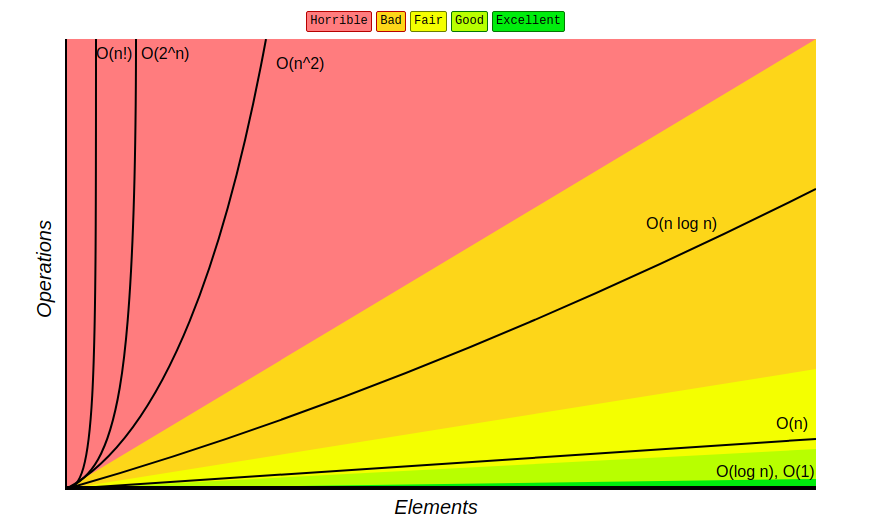
\includegraphics[width=1\linewidth]{screenshot002}
			\caption[Gráfico de complexidade Big-O]{Gráfico de complexidade Big-O}
			\label{fig:screenshot002}
		\end{figure}
		\begin{figure}
			\centering
			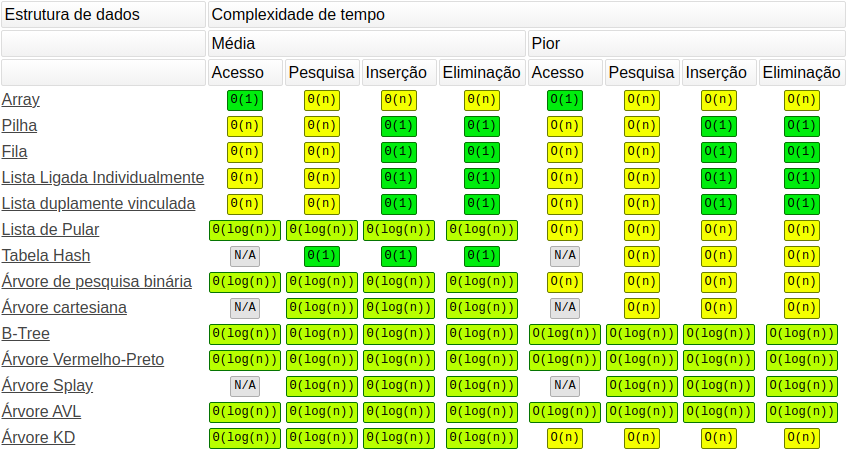
\includegraphics[width=1\linewidth]{screenshot003}
			\caption[Operações comuns de estrutura de dados]{Operações comuns de estrutura de dados}
			\label{fig:screenshot003}
		\end{figure}
\end{center}
	\newpage

	\subsection{SHA-1}
O termo Secure Hash Algorithm ( SHA , Inglês para algoritmo de hash seguro ) descreve um grupo de padronizados funções hash criptográficas .Eles são usados para calcular um valor de teste para quaisquer dados digitais (mensagens) e são, entre outras coisas, a base para a criação de uma assinatura digital .
	
	As funções hash criptográficas são projetadas para aceitar strings de comprimento arbitrário como entrada e gerar valores hash de comprimento fixo. A função hash criptográfica deve ser capaz de resistir a todos os ataques de análise criptográfica conhecidos. 
	
	 No mínimo, ele deve ter os seguintes atributos: 
	  \begin{itemize}
	 	\item Resistência à pré-imagem:
	 	Dado um valor hash h deve ser difícil encontrar qualquer mensagem m tal que h = hash(m). Este conceito está relacionado ao da função de mão única (ou função unidirecional). Funções que não possuem essa propriedade estão vulneráveis a ataques de pré-imagem.
	 	\item Resistência à segunda pré-imagem:
	 	Dada uma entrada m1 deve ser difícil encontrar outra entrada m2 tal que hash(m1) = hash(m2). Funções que não possuem essa propriedade estão vulneráveis a ataques de segunda pré-imagem.
	 	\item Resistência à colisão:
	 	Deve ser difícil encontrar duas mensagens diferentes m1 e m2 tal que hash(m1) = hash(m2). Tal par é chamado de colisão hash criptográfica. Essa propriedade também é conhecida como forte resistência à colisão. Ela requer um valor hash com pelo menos o dobro do comprimento necessário para resistência à pré-imagem; caso contrário, colisões podem ser encontradas através de um ataque do aniversário.
	 \end{itemize}
	  
	  
	  Por serem um tipo específico de função hash, as funções hash criptográficas também são muito adequadas para ser utilizadas para indexar dados em tabelas hash.
	
	  No entanto, em comparação com as funções hash padrão, as funções hash criptográficas costumam ser muito mais caras em termos computacionais. Portanto, eles tendem a ser 
	usados onde os usuários precisam se proteger
	   da possibilidade de falsificação por usuários mal-intencionados em potencial.
	  
	\newpage

	
	\addcontentsline{toc}{section}{Bibliografia}
	\section*{Bibliografia}

\footnotesize{
	\noindent Mark Allen Weiss. Data Structure and Algorithms in C++, chapter Chapter 5 – Hashing, pages 193–244. Pearson Education, Inc. as Addison-Wesley, 2014.\\

}
\footnotesize{
	
	\noindent https://www.bigocheatsheet.com/\\
	
}


\end{document}



